\chapter{GIẢI PHÁP HẠN CHẾ THIỆT HẠI DO THÔNG TIN SAI LỆCH GÂY RA TRÊN MẠNG XÃ HỘI}

\section{Đặt vấn đề, định nghĩa bài toán}
Tự do ngôn luận, tự do báo chí là một trong những quyền căn bản của công dân đã được Hiến pháp ghi nhận và đã được Đảng và Nhà nước nhất quán. Tuy nhiên thực tế hiện nay có rất nhiều cá nhân, tổ chức đã và đang lợi dụng các quyền này để xâm phạm lợi ích của Nhà nước và lợi ích chính đáng của công dân. Với sự phát triển mạnh mẽ của Internet và mạng xã hội trực tuyến, việc đăng tải, tuyên truyền các thông tin sai lệch mang tính chất xuyên tạc, chống đối đường lối chính sách của Đảng, pháp luật của Nhà nước, hoạt động của bộ máy chính quyền diễn ra thường xuyên hơn với âm mưu, quy mô và tổ chức ngày càng rộng lớn, chặt chẽ.

Như thường lệ, mỗi khi cơ quan chức năng Việt Nam tiến hành truy tố, xét xử những cá nhân có hành vi vi phạm pháp luật như: Hoạt động nhằm lật đổ chính quyền nhân dân (theo Điều 109 Bộ luật Hình sự năm 2015, sửa đổi bổ sung năm 2017); tuyên truyền chống Nhà nước Cộng hòa XHCN Việt Nam (Điều 117) hay lợi dụng các quyền tự do, dân chủ, xâm phạm lợi ích của Nhà nước, quyền, lợi ích hợp pháp của tổ chức, công dân (Điều 331) thì ngay lập tức một số tổ chức, cá nhân chống đối trong và ngoài nước lại ráo riết tuyên truyền xuyên tạc, chống phá Việt Nam trên lĩnh vực dân chủ, nhân quyền. Những đối tượng này đã lợi dụng quyền tự do ngôn luận để viết và đăng tải các nội dung sai lệch, không có căn cứ, tuyền truyền xuyên tạc đường lối, chính sách của Đảng, pháp luật của Nhà nước, bôi nhọ các cán bộ, Đảng viên làm ảnh hưởng đến uy tín của cơ quan, tổ chức, đi ngược lại với lợi ích quốc gia, dân tộc.

Xuất phát từ những thực tế nêu trên, nhóm tác giả nhận thấy việc nghiên cứu đề ra giải pháp ngăn chặn kịp thời sự lan truyền của thông tin sai lệch trên MXH là một thách thức lớn cần giải quyết kịp thời. Tuy nhiên trong quá trình nghiên cứu, nhóm tác giả đã gặp phải một số vấn đề khó khăn.

Theo Điều 22, Luật An ninh Quốc gia nước Cộng hòa xã hội chủ nghĩa Việt Nam năm 2004, Công An nhân dân mà một trong các cơ quan chuyên trách được giao thực hiện nhiệm vụ bảo vệ An ninh quốc gia. Theo Điều 10, Luật Viễn thông năm 2009 quy định Cơ quan quản lý chuyên ngành về viễn thông là cơ quan thuộc Bộ Thông tin và Truyền thông. Tuy nhiên trong thực tế, các cơ quan chức năng của Nhà nước ta chưa có quyền quản lý đối với các nội dung trên mạng xã hội, được quản lý bởi các tập đoàn Facebook, Twitter, Microsoft. Do đó, việc xóa bỏ các nội dung, thông tin sai lệch lan truyền trên mạng xã hội, hay vô hiệu hóa người dùng đăng tải thông tin sai lệch là không khả thi. 

Một vấn đề đặt ra khác là, các thông tin sai lệch phán tán trên mạng xã hội xuất phát từ các nguồn phát tán với tốc độ nhanh, quy mô rộng lớn. Đã có nhiều nghiên cứu đưa ra nhằm xác định các nguồn phát tán này, tuy nhiên hiệu quả và độ chính xác vẫn còn nhiều hạn chế. Trong thực tế, các nguồn phát tán thông tin sai lệch, các thông tin chống đối và xuyên tạc chính sách, đường lối của Đảng, pháp luật của Nhà nước thường là các đối tượng chủ mưu, cầm đầu, nắm vai trò quan trọng trong các tổ chức phản động. Đây là những đối tượng cơ hội chính trị, đối tượng bất mãn, đối tượng bảo thủ, ngoan cố và rất khó để thuyết phục các đối tượng đó gỡ bỏ các bài đăng, thông tin sai lệch trên mạng xã hội.

Trong nghiên cứu này, nhóm tác giả đã dùng phương pháp giám sát, điều tra để tìm ra những đối tượng có tính chất trên, coi họ là nguồn phát tán thông tin sai lệch. Sau đó, nhóm tác giả đã nghiên cứu và đề xuất giải pháp chọn ra tập người dùng để vô hiệu hóa họ trong việc tham gia vào quá trình phát tán thông tin sai lệch. Trên mạng xã hội, hoạt động này tương đương với các biện pháp như sau:
\begin {itemize}
	\item Thuyết phục người dùng không chấp nhận và lan truyền những thông tin sai lệch đến những người dùng khác, tức là làm cho người dùng này không tham gia vào quá trình phát tán thông tin sai lệch. Kĩ thuật này, ở trong các nghiên cứu gần đây còn được gọi là đặt giám sát (Monitor) người dùng \cite{zhang32}, \cite{zhang33}, \cite{zhang34}.

	\item Bằng sự can thiệp và giúp đỡ của nhà mạng có thể loại bỏ, cách ly thông tin sai lệch đến với những người dùng này. Năm 2016, Twitter đã loại bỏ 125.000 tài khoản được nghi ngờ có liên quan đến các hoạt động khủng bố \cite{twitter}. Năm 2017, Facebook đã xóa 30.000 tài khoản giả mạo lan truyền các tin đồn trước cuộc bầu cử tổng thống Pháp năm 2017 \cite{french}.
\end {itemize}

Dưới những điều kiện khác nhau, như tiềm lực tài chính, khả năng thuyết phục, phạm vi lan truyền thông tin khác nhau, cùng với đó là các mục tiêu khác nhau, có thể kể đến ảnh hưởng lan truyền của thông tin sai lệch, tỉ lệ người dùng nhiễm thông tin sai lệch và với các mô hình lan truyền thông tin khác nhau. Nhóm tác giả đã tiến hành thu thập dữ liệu trực tiếp từ mạng xã hội Facebook, với phạm vi xung quanh các đối tượng chống đối, đối tượng cầm đầu trong thời gian gần đây, sau đó mô hình hóa các dữ liệu thu được, và nghiên cứu lý thuyết, đề xuất hai giải pháp ngăn chặn hiệu quả, tiến hành thực nghiệm và so sánh với các giải pháp đã công bố trước đây. 

Kết quả cuối cùng của giải pháp đưa ra một danh sách người dùng tiềm năng, theo đánh giá về lý thuyết và thực nghiệm cho thấy, nếu dùng các biện pháp ngăn chặn nêu trên để vô hiệu hóa những người dùng này, ảnh hưởng của những thông tin sai lệch đối với mạng xã hội là nhỏ hơn những giải pháp đã được công bố trước đây, và thời gian thực hiện các giải pháp của nhóm tác giả là tương đối nhanh.

\section{Tổng thể về giải pháp}
Giải pháp ngăn chặn thông tin sai lệch trên MXH được nhóm tác giả thực hiện qua 4 bước. Đầu tiên là quá trình giám sát, điều tra để thu thập được tài khoản mạng xã hội của những đối tượng chủ mưu, cầm đầu các tổ chức phản động, các đối tượng có uy tín lớn. Sau đó nhóm tác giả sử dụng công cụ kiểm thử Selenium để thu thập mạng xã hội xung quanh các đối tượng này. Bước tiếp theo, nhóm tác giả mô hình hóa toán học mạng xã hội thực thu được ở bước trên, và cuối cùng đề xuất, áp dụng hai giải pháp hiệu quả, để đưa ra tập người dùng tiềm năng có thể áp dụng các biện pháp vô hiệu hóa để ảnh hưởng của thông tin sai lệch trên mạng là nhỏ nhất.

MXH cho phép các nhà phát triển (Developers) có thể lấy được thông tin dữ liệu, tuy nhiên điều đó phải được sự cho phép của người dùng thông qua các mã truy cập Access Token (Access Token là một đoạn mã do MXH sinh ra ngẫu nhiên khi người dùng đồng ý cho ứng dụng thứ 3 thực hiện các thao tác đối với tài khoản của người dùng). Điều này là một vấn đề khó khăn khi chúng ta cần khảo sát, lấy thông tin đối với một số lượng lớn người dùng nhằm xây dựng được đồ thị quan hệ giữa các người dùng trên MXH.

Nhằm giải quyết vấn đề trên, nhóm tác giả đề xuất một hướng tiếp cận mới là sử dụng công cụ kiểm thử phần mềm tự động mã nguồn mở Selenium cho việc kiểm thử ứng dụng Web. Cụ thể ở đây nhóm tác giả thư viện mã nguồn mở của Selenium trên ngôn ngữ Python, kiểm thử tự động với trình duyện Chromnium.
	\subsection{Công cụ kiểm thử Selenium}
	Selenium là một công cụ kiểm thử phần mềm tự động, được phát triển bởi ThoughtWorks từ năm 2004 với tên ban đầu là JavaScriptTestRunner. Đến năm 2007, tác giả Jason Huggins rời ThoughtWorks và gia nhập Selenium Team, một phần của Google và phát triển thành Selenium như hiện nay.
	
	Selenium cung cấp công cụ phát lại (Playback) cho việc tạo ra các bài kiểm thử mà không cần phải học một ngôn ngữ kịch bản khác (Selenium IDE). Nó cũng cung cấp một ngôn ngữ thử nghiệm tên miền cụ thể (Selenese) để tạo ra các bài kiểm thử bằng một số ngôn ngữ lập trình phổ biến bao gồm C\#, Groovy, Java, Perl, Python, PHP, Ruby, Scala. Các thử nghiệm sau đó có thể chạy trên hầu hết các trình duyệt Web hiện đại. Selenium triển khai trên các nền tảng Windows, Linux và cả MacOS. Selenium là phần mềm mã nguồn mỡ, được phát hành theo giấy phép Apache 2.0.
	
	Selenium bao gồm một số thành phần với mỗi thành phần tham gia vào một vai trò cụ thể trong việc hỗ trợ phát triển tự động kiểm tra ứng dụng Web.
		\subsubsection{IDE Selenium}
		Là một môi trường phát triển tích hợp hoàn chỉnh (IDE) cho các bài kiểm tra Selenium. Nó được thực hiện như một Tiện ích bổ sung của Firefox và cho phép ghi lại, chỉnh sửa và gỡ lỗi. Nó trước đây được gọi là Selenium Recorder. Selenium-IDE ban đầu được tạo ra bởi Shinya Kasatani và được tặng cho dự án Selenium vào năm 2006. Nó ít được duy trì và tương thích với Selenium RC. Các tập lệnh có thể tự động được ghi lại và chỉnh sửa theo cách thủ công, cung cấp hỗ trợ tự động hoàn thành và khả năng di chuyển các lệnh nhanh chóng. Kịch bản được ghi lại trong Selenese ,một ngôn ngữ kịch bản thử nghiệm đặc biệt cho Selenium. Selenese cung cấp các lệnh để thực hiện các hành động trong một trình duyệt (bấm vào một liên kết, chọn một tùy chọn) và để lấy dữ liệu từ các trang kết quả.
		\subsubsection{API Client Selenium}
		Để thay thế cho các bài kiểm tra viết bằng Selen, các bài kiểm tra cũng có thể được viết bằng nhiều ngôn ngữ lập trình khác nhau. Những thử nghiệm này sau đó giao tiếp với Selenium bằng cách gọi các phương thức trong API ứng dụng khách Selenium. Selenium hiện cung cấp các API ứng dụng khách cho Java , C\#, Ruby , JavaScript và Python. Với Selenium 2, một API ứng dụng khách mới đã được giới thiệu (với WebDriver là thành phần trung tâm của nó). Tuy nhiên, API cũ (sử dụng lớp Selenium) vẫn được hỗ trợ.
		\subsubsection{Selenium WebDriver}
		Selenium WebDriver là sự kế thừa của Selenium RC. Selenium WebDriver chấp nhận các lệnh (được gửi bằng Selenese hoặc thông qua API ứng dụng khách) và gửi chúng tới trình duyệt. Điều này được thực hiện thông qua trình điều khiển trình duyệt cụ thể cho trình duyệt, trình điều khiển sẽ gửi lệnh tới trình duyệt và truy xuất kết quả. Selenium WebDriver không cần một máy chủ đặc biệt để thực hiện các thử nghiệm. Thay vào đó, WebDriver trực tiếp khởi động một cá thể trình duyệt và điều khiển nó. Tuy nhiên, Selenium Grid có thể được sử dụng với WebDriver để thực hiện các kiểm tra trên các hệ thống từ xa. Nếu có thể, WebDriver sử dụng chức năng cấp hệ điều hành gốc hơn là các lệnh JavaScript dựa trên trình duyệt để điều khiển trình duyệt. Điều này bỏ qua các vấn đề với sự khác biệt tinh tế giữa lệnh gốc và JavaScript, bao gồm cả các hạn chế bảo mật.
		\subsubsection{Selenium remote control}
		Selenium Remote Control (RC) là một máy chủ, được viết bằng Java, chấp nhận các lệnh cho trình duyệt thông qua HTTP. RC giúp có thể viết các bài kiểm tra tự động cho một ứng dụng web bằng bất kỳ ngôn ngữ lập trình nào, cho phép tích hợp tốt hơn Selenium trong các khung kiểm thử đơn vị hiện có. Để làm cho các bài kiểm tra viết dễ dàng hơn, dự án Selenium hiện cung cấp các trình điều khiển máy khách cho PHP, Python, Ruby, .NET, Perl và Java.
		\subsubsection{Selenium Grid}
		Selenium Grid là một máy chủ cho phép kiểm tra sử dụng các cá thể trình duyệt web chạy trên các máy từ xa. Với Selenium Grid, một máy chủ hoạt động như một hub. Kiểm tra liên hệ với trung tâm để có được quyền truy cập vào các phiên bản trình duyệt. Trung tâm có một danh sách các máy chủ cung cấp quyền truy cập vào các cá thể của trình duyệt (các nút WebDriver) và cho phép các thử nghiệm sử dụng các cá thể này. Selenium Grid cho phép chạy thử nghiệm song song trên nhiều máy và quản lý các phiên bản trình duyệt khác nhau và cấu hình trình duyệt tập trung (thay vì trong từng thử nghiệm riêng lẻ).
	
	\subsection{Kĩ thuật lấy dữ liệu trên MXH}
	\begin{center}
		\begin{figure}[htp]
			\begin{center}
				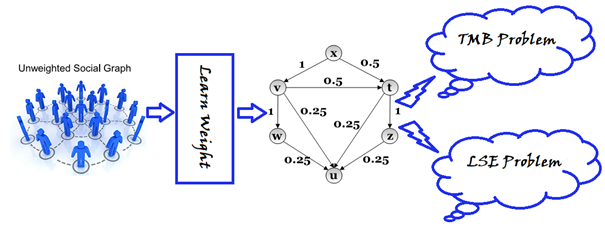
\includegraphics [scale=.5]{picture/Hinh3_1}
			\end{center}
			\caption{Quá trình lấy dữ liệu}
			\label{refhinh3_1}
		\end{figure}
	\end{center}
	Quá trình lấy dữ liệu, áp dụng để xử lý được mô tả thông qua mô hình ở Hình \ref {refhinh3_1}.
		\subsubsection{Thu thập dữ liệu từ MXH Facebook}
		Các bước cụ thể của giai đoạn thu thập dữ liệu trên MXH Facebook được mô tả cụ thể như sau:
		\begin {itemize}
			\item Đầu tiên, nhóm tác giả tạo một tài khoản Facebook rồi sử dụng Công cụ kiểm thử tự động Selenium để tự động đăng nhập vào tài khoản Facebook đó.
		
			\item Bằng các truy vấn đặc biệt, nhóm tác giả lấy được ID (Identity Number) của tài khoản trên.
		
			\item Thông qua phương pháp giám sát và điều tra, thông qua những tin tức, vụ việc trong thời gian gần đây. Nhóm tác giả khảo sát dữ liệu với tập nguồn ban đầu bao gồm 6 tài khoản Facebook, đây là các đối tượng chủ mưu, cầm đầu, nắm vai trò quan trọng trong các tổ chức phản động, thường xuyên có các bài viết, bình luận mang tính chất chống đối, và đặc biệt các đối tượng này có uy tín khá lớn, có lượng người theo dõi, bạn bè trên Facebook là vô cùng đông đảo.
			\begin {enumerate} [+]
				\item https://www.facebook.com/gioan.namphong: Linh mục giáo sứ Thái Hà Nguyễn Nam Phong, một nhân vật khá nổi tiếng trong làng chống chính quyền trong nước và thường xuyên ra nước ngoài để "liên lạc" với tổ chức khủng bố Việt Tân.
		
				\item https://www.facebook.com/minhnhat.paultran: Paul Trần Minh Nhật là giáo dân thuộc xứ Ngọc Long, xã Công Thành, Yên Thành, Nghệ An, từng bị bắt và kết án 4 năm tù về tội “hoạt động nhằm lật đổ chính quyền nhân dân”. Hiện tại, Minh Nhật đang là cộng tác viên của trang “Tin mừng cho người nghèo”, mang danh nghĩa rao giảng tin mừng của Chúa, nhưng lại nhuốm màu sắc chính trị, luôn ủng hộ các đối tượng vi phạm pháp luật.
		
				\item https://www.facebook.com/ThaiDung2016: Gioan Thái Văn Dung là sinh viên tốt nghiệp ngành tin học, đã tham gia quản lý cửa hàng Internet, Do hiểu biết được CNTT mà biết thêm về xã hội, tích cực truyền bá thông tin, hoạt động mạng, tham gia biểu tình chống TQ xâm lược.
		
				\item https://www.facebook.com/pham.doan.trang: Nhà báo Phạm Đoan Trang, từng công tác tại Báo Pháp Luật thành phố Hồ Chí Minh. Tác giả của cuốn sách “Chính trị Bình Dân” có những nội dung nhạy cảm, mang tính chất kích động, chống phá chính quyền, Đảng và Nhà Nước.
		
				\item https://www.facebook.com/jbnguyenhuuvinh: Anh Ba Sàm, tên thật là Nguyễn Hữu Vinh là một blogger, từng là công an và đảng viên Đảng Cộng sản Việt Nam, từng công tác ở Ủy ban Việt kiều Trung ương. Ông bị Chính phủ CHXHCN Việt Nam bắt giữ và bị cáo buộc và phạt tù 5 năm do có hành vi đăng tải các bài viết trên mạng Internet vi phạm Điều 258 Bộ Luật Hình sự năm 2015 sửa đổi bổ sung năm 2017 về Tội lợi dụng các quyền tự do dân chủ xâm phạm lợi ích của Nhà nước, quyền, lợi ích hợp pháp của tổ chức, công dân.
		
				\item https://www.facebook.com/profile.php?id=100015485029386: Nguyễn Trọng đang sinh sống tại California, Hoa Kỳ. Lợi dụng quyền tự do dân chủ, thường xuyên có những bài viết xuyên tạc, chống phá đường lối chính sác của Đảng, pháp luật của Nhà nước.
				\end {enumerate}
			\item Tiếp theo, nhóm tác giả tự động trup cập vào trang web có địa chỉ www.facebook.com/{ID}/friends hoặc www.facebook.com/{name}/friends là trang bạn bè của những người dùng đó.
		
			\item Theo thuật toán sắp xếp của Facebook, những người dùng có liên quan nhất và hay tương tác nhất với người dùng đang theo dõi sẽ hiện ra đầu tiên trong trang bạn bè nói trên. Nhóm tác giả sử dụng thư viện BeautifulSoup để lấy mã HTML của trang này, tìm và lấy các đường dẫn chứa địa chỉ Facebook bạn bè của người dùng đang theo dõi, lấy ID của họ.
		
			\item Nhóm tác giả thu thập theo phương pháp loang theo chiều rộng: Bắt đầu từ ID Facebook của 6 đối tượng kể trên, từ đó tìm tiếp thông tin về khoảng 20 người bạn xuất hiện đầu tiên trên trang Facebook bạn bè của mỗi người dùng đó. Với mỗi người dùng thu thập được, nhóm tác giả lại tiếp tục tiến hành thu thập như trên, và cứ tiếp tục tìm kiếm đến khi thu thập đủ số lượng người dùng cần thiết.
		\end {itemize}		
		Cách làm này có ưu điểm là những người dùng thu thập được có nhiều mối liên hệ với nhau, đồ thị MXH thu thập được có nhiều liên kết, mang lại sự trực quan hơn cho cấu trúc đồ thị mạng. Ngoài ra còn có quá trình tiền xử lý, bước này sẽ hạn chế, loại bỏ được những đỉnh cô lập, hay những đỉnh khai thác được ít thông tin (Không công khai danh sách bạn bè).
		
		Bên cạnh những ưu điểm trên, thì cách làm này cũng có nhược điểm là không khai thác được hết thông tin của người dùng, bởi nhiều người dùng không để chế độ công khai bạn bè. Trong thực tế sẽ để lọt nhiều đối tượng nguy hiểm, ẩn chứa nhiều nguy cơ tiềm tàng.
		
		\subsubsection{Mô hình hóa dữ liệu thu được}
		Ở bước này, từ những dữ liệu thu thập được về danh sách ID người dùng, mối quan hệ bạn bè giữa họ. Nhóm tác giả tiền xử lý, đánh số lại các đỉnh, xây dựng đồ thị mô tả MXH với các đỉnh đại diện cho các người dùng, các cạnh biểu diễn mối quan hệ bạn bè giữa những người đó, trọng số (nếu có) đại diện cho mức độ tương tác giữa người dùng với nhau. Kết quả đầu ra của thuật toán thu thập thông tin trên MXH Facebook bao gồm 2 file dữ liệu:
		\begin {itemize}
			\item ID.txt chứa ánh xạ từ ID của người dùng sang chỉ số đỉnh được đánh số lại. Qua quá trình thu thập dữ liệu, chuẩn hóa, nhóm tác giả thu được 542 ID người dùng, được đánh số lại từ 0 – 541, xem bảng \ref{bang3_1}		
		\begin{table} [!htp]
			\centering 
			\begin{tabular}{|c|c|}
			\hline 
			0 & 100003708850657 \\ 
			\hline 
			1 & 100009945675640 \\ 
			\hline 
			2 & 100010197936720 \\ 
			\hline 
			3 & 641613321 \\ 
			\hline 
			4 & 100002541019308 \\ 
			\hline 
			5 & 100015485029386 \\ 
			\hline 
			6 & 100004745583805 \\ 
			\hline 
			... & ... \\ 
			\hline 
			539 & 100004236103486 \\ 
			\hline 
			540 & 100004142778267 \\ 
			\hline 
			541 & 100006259445960 \\ 
			\hline 
			\end{tabular} 
			\caption{Ví dụ ánh xạ ID người dùng sang chỉ số được đánh số.}
			\label{bang3_1}
		\end{table}
		 	\item Network.txt chứa mô tả cụ thể của đồ thị MXH đã thu được. File dữ liệu gồm nhiều dòng, mỗi dòng chứa 2 số là chỉ số của 2 người dùng có quan hệ với nhau.
		 
		 \begin{table} [!htp]
		 	\centering
		 	\begin{tabular}{|c|c|}
		 	\hline 
		 	0 & 7 \\ 
		 	\hline 
		 	0 & 8 \\ 
		 	\hline 
		 	0 & 9 \\ 
		 	\hline 
		 	0 & 4 \\ 
		 	\hline 
		 	... & ... \\ 
		 	\hline 
		 	99 & 400 \\ 
		 	\hline 
		 	99 & 437 \\ 
		 	\hline 
		 	99 & 498 \\ 
		 	\hline 
		 	\end{tabular}
	 		\caption{Mô tả cụ thể của đồ thị MXH thu được}
	 		\label{bang3_2} 
		 \end{table}
	 
	 	Từ dữ liệu thu được, nhóm tác giả mô phỏng lại và thu được hình ảnh tổng quan về cấu trúc mạng như sau :
	 
	 	\begin{center}
	 		\begin{figure}[htp]
	 			\begin{center}
	 				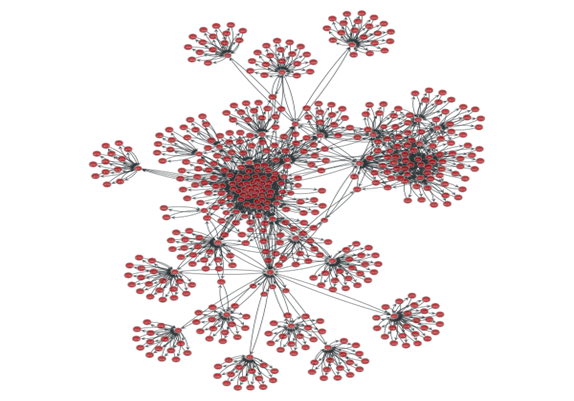
\includegraphics [scale=.5]{picture/Hinh3_2}
	 			\end{center}
	 			\caption{Mô phỏng cấu trúc toàn mạng dữ liệu thu được}
	 			\label{refhinh3_2}
	 		\end{figure}
	 	\end{center}
 	\end {itemize}
 	\subsection{Giải pháp hạn chế: Limiting the spread of epidemics within time constraint on online social network (Ngăn chăn khả năng lan truyền của thông tin sai lệch trong thời gian giới hạn trên một mạng xã hội)}
 	Giải pháp này được đề xuất và nghiên cứu sau khi xem xét thực tế quá trình lan truyền của một thông tin sai lệch trên mạng xã hội. Thông tin sai lệch luôn bắt đầu từ một số người dùng nhất định (có thể coi như đỉnh “nguồn” phát tán thông tin sai lệch). Những người dùng này thường là những tên có tư tưởng lệch lạc, phản động, và thông tin sai lệch thường là những thông tin bị bóp méo, những sai lầm của cán bộ bị thồi phồng, hoặc những lời lẽ bịa đặt vô căn cứ. Từ những người dùng bắt đầu này, thông tin sẽ được biết đến bởi những người xung quanh có liên kết với chúng, thường là những người dùng có quan hệ bạn bè với chúng. Thông tin này ban đầu có thể không tác động tới người dùng xung quanh, tuy nhiên nếu nó xuất hiện thêm nhiều lần từ nhiều nguồn khác nhau thì họ có thể sẽ tiếp nhận thông tin đó, và từ đó trở thành một nguồn phát thông tin sai lệch mới. Nếu mọi việc cứ phát triển thì thông tin này dần dần sẽ lan truyền sang toàn bộ một cộng đồng, hoặc thậm chí là toàn mạng xã hội (Quá trình lan truyền này được biểu diễn thông qua mô hình lan truyền được định nghĩa bên dưới). Do đó, cần có phương pháp giúp kiểm soát tình hình, ngăn chặn thông tin sai lệch lan truyền quá rộng, và đây cũng là lí do mà giải pháp này được nghiên cứu và công bố. Giải pháp được thiết kế để có thể chọn một số người dùng đặc biệt. Những người dùng được chọn này sau đó sẽ được các cơ quan chức năng có thẩm quyền tiến hành các phương pháp phù hợp đề ngăn chặn khả năng phát tán thông tin của họ. Từ đó, thông tin sai lệch sẽ không có khả năng truyền thông qua những người dùng này, và dẫn đến khả năng lan truyền sang những người dùng tiếp theo bị cản trở. Giải pháp này đã được chứng minh rằng nó có thể lựa chọn ra các đỉnh hiệu quả nhất để ngăn chặn, do đó vừa đem lại hiệu quả cao mà không hao tốn quá nhiều tài nguyên vào việc ngăn chặn các đỉnh kém hiệu quả khác.
 		\subsubsection{Mô hình lan truyền thông tin Ngưỡng tuyến tính với bước thời gian rời rạc (Time Constraint Deterministic Linear Threshold - T-DLT).}
 		Như đã được trình bày ở trên, có hai mô hình phổ biến trong bài toán lan truyền thông tin nói chung là mô hình IC và mô hình LT. Tuy nhiên, ở giải pháp này chúng tôi đề xuất một mở rộng mô hình DLT \cite{zaixin}, vốn cũng là một trường hợp biến thể của mô hình LT, được gọi là T-DLT. Sở dĩ chúng tôi sử dụng mô hình này thay cho mô hình LT và IC bởi với bài toán này, mô hình T-DLT cho phép chúng tôi giảm thiểu tính phức tạp của cơ chế lan truyền, đồng thời vẫn đảm bảo kết quả không bị ảnh hưởng so với hai mô hình điển hình trên. Chi tiết mô hình T-DLT có thể được mô tả như sau:
 		\begin {itemize}
 			\item {\itshape Ký pháp đồ thị}: Đặt G=(V,E,w) là biểu diễn của MXH với tập đỉnh V, tập cạnh có hướng E, với |V|=n và |E|=m. Mỗi đỉnh đại diện cho một người dùng trong MXH, mỗi cạnh e=(u,v) trong tập E tương ứng đại diện cho mỗi quan hệ giữa người dùng u và người dùng v. Chúng tôi ký hiệu đỉnh vào liền kề và đỉnh ra liền kề của đỉnh u lần lượt là N$_{in}$(u) và N$_{out}$(u), d$_{in}$(u) và d$_(out)$(u) lần lượt là bậc vào và bậc ra của đỉnh u. Đặt I $\subset$ V là tập các đỉnh bị lây nhiễm ban đầu. Mỗi cạnh có hướng (u,v) sẽ có trọng số w(u,v), tượng trưng cho mức độ ảnh hưởng thông tin của v tới u, thỏa mãn $\sum$ $_(u)$ w(u,v) $\leq$ 1.
 		
 			\item {\itshape Trạng thái của đỉnh}: Quá trình phát tán thông tin sai lệch từ tập đỉnh ban đầu I tới các đỉnh còn lại trong MXH tiến triển theo từng bước thời gian rời rạc t=1,2,…,d. Mỗi đỉnh v $\in$ V có hai trạng thái là {\itshape bị lây nhiễm (hay “kích hoạt”)} và {\itshape không bị lây nhiễm (hay “không kích hoạt”)}.
 		
 			\item {\itshape Ngưỡng lây nhiễm (hay ngưỡng kích hoạt)}: Mỗi đỉnh v sẽ có một ngưỡng lây nhiễm cho trước $\theta$$_(v)$ $\in$ [0,1]. Giá trị này đại diện cho trọng số vào của đỉnh v cần chuyển thành bị lây nhiễm để v trở thành bị lây nhiễm.
 		
 			\item {\itshape Quá trình lan truyền}: Quá trình lây lan thông tin sai lệch được mô phỏng tuần tự theo từng bước thời gian rời rạc (còn gọi là $``$vòng$"$, $``$bước$"$) t=0,1,2,…,d. Đặt I$_(t)$ là tập các đỉnh bị lây nhiễm sau t bước, quá trình lan truyền được mô phỏng như sau:
 			\begin {enumerate} [+]
 				\item Tại bước t=0, tất cả các đỉnh trong tập I đều bị lây nhiễm, I$_(0)$=I.
 		
 				\item Tại bước t $\geq$ 1, tất cả các đỉnh không bị lây nhiễm v sẽ chuyển thành bị lây nhiễm nếu tổng số các đỉnh vào gần kề chạm ngưỡng lây nhiễm của nó, $\sum$$_(các đỉnh vào gần kề của u)$ w(u,v) $\geq$ $\theta$$_(v)$.	
 		
 				\item Một đỉnh bị lây nhiễm sẽ giữ nguyên trạng thái bị lây nhiễm cho tới hết quả trình lan truyền. Qúa trình lan truyền chấm dứt khi t = d.
 			\end {enumerate}
 		\end {itemize}
 		Trong mô hình LT, giá trị của ngưỡng $\theta$$_(v)$ được đặt một cách ngẫu nhiên trong khoảng [0,1] và sẽ được chỉnh sửa dựa vào thông tin có được thêm trong quá trình lan truyền. Do đó, mô hình này thuộc dạng mô hình ngẫu nhiên. Khác với mô hình LT, trong mô hình T-DLT ngưỡng lây nhiễm $\theta$$_(v)$ được cho trước. Trường hợp này, giá trị ngưỡng có thể được đặt dựa theo các khảo sát thực tế hoặc các phương pháp khai phá dữ liệu.
 		
 		\subsubsection{Định nghĩa bài toán}
 		Đối với giải pháp này, việc ngăn chặn thông tin sai lệch được tiến hành bằng cách loại bỏ một số người dùng ra khỏi mạng để thông tin không thể truyền qua được, sao cho phạm vi lan truyền của thông tin là nhỏ nhất có thể. Nếu như coi mạng xã hội là một đồ thị, thì ta có thể hiểu rằng những đỉnh $``$bị lây nhiễm$”$ là những người dùng đã bị ảnh hưởng bởi thông tin sai lệch và thông tin sai lệch đó có thể truyền từ người dùng này sang những người dùng thân cận, những đỉnh $``$không bị lây nhiễm$”$ là những đỉnh không bị ảnh hưởng bởi thông tin sai lệch, còn những đỉnh $``$cứu được$”$ là những đỉnh mà có trạng thái chuyển từ $``$bị lây nhiễm$”$ sang $``$không bị lây nhiễm$”$ khi chiến thuật loại bỏ đỉnh được áp dụng. Trong thực tế, việc loại bỏ một người dùng ra khỏi mạng xã hội có thể được thực hiện bằng cách thuyết phục người dùng đó thoát khỏi sự ảnh hưởng của thông tin sai lệch, hoặc ngăn chặn kết nối mạng của người dùng đó, hoặc xóa bỏ tài khoản của người dùng ra khỏi mạng xã hội, v.v… Tuy nhiên, những cách làm này đều là những cách làm yêu cầu có sự phối hợp từ nhiều bên liên quan, do đó nếu tiến hành loại bỏ quá nhiều sẽ dẫn đến chi phí phát sinh về thời gian và vật chất rất lớn, thậm chí sẽ gây ra trường hợp loại bỏ những thông tin lan truyền quá rộng dẫn đến vô ích. Vì vậy, vấn đề đặt ra là phải làm sao chọn ra được một số lượng K đỉnh nào đó để khi thực hiện chiến thuật loại bỏ, ta thu được số đỉnh cứu nhiều nhất. Số lượng K sẽ được tính toán một cách cân đối, cẩn thận nhất về chi phí để không làm mất tác dụng của chiến thuật loại bỏ. Chiến thuật loại bỏ K đỉnh này có thể được mô hình hóa và phát biểu khoa học như sau:  
 		
 		Kí hiệu f$_{d}$(I) là tập hợp các đỉnh đã bị lây nhiễm sau d vòng trên đồ thị G = (V,E) trong mô hình T-DLT, f$_(d)$(I,A) là tập các đỉnh bị lây nhiễm sau khi loại bỏ một tập các đỉnh A $\subseteq$ V \ I từ G (số đỉnh bị lây nhiễm trong đồ thị sót lại). Khi đó, số đỉnh cứu được khi loại bỏ tập A là: h$_{d}$(A) = | f$_{d}$(I, $\emptyset$) | - | f$_{d}$(I, A) |
 		
 		Trong mô hình T-DLT, ta xây dựng một bài toán tối ưu tổ hợp là: {\itshape Hạn chế sự lây lan của thông tin sai lệch} (Limiting the Spread of Epidemics - LSE), có mục tiêu tìm kiếm một tập đỉnh có kích cỡ tối đa k đỉnh sao cho khi loại bỏ tập đỉnh đó, số đỉnh cứu được sẽ đạt cực đại.  
 		
 		{\itshape Định nghĩa (Bài toán LSE): Cho đồ thị vô hướng G=(V,E) biểu diễn một MXH trong mô hình T-DLT. Một tập các đỉnh bị lây nhiễm ban đầu I $\subset$ V, số vòng lan truyền d và số đỉnh tối đa loại bỏ được là k > 0. Tìm một tập k đỉnh  A $\subseteq$ V \ I sao cho khi loại bỏ khỏi mạng thì số đỉnh cứu được sau d vòng là h$_{d}$(A) đạt cực đại.}
 		
 		Kí hiệu G$_{d}$ = (V$_{d}$, E$_{d}$) đồ thị con của đồ thị G=(V, E) trong đó V$_{d}$ là tập các đỉnh mà khoảng cách giữa một đỉnh bất kì trong đó với một đỉnh trong tập I tối đa là d, và tập E$_{d}$ là tập các cạnh nối từ các đỉnh thuộc tập I sang các đỉnh khác có khoảng cách tối đa là d, đồng thời n$_{d}$ = | V$_{d}$ |, m$_{d}$ = | E$_{d}$ |. Ta thấy rằng sự lan truyền thông tin sai lệch chỉ xảy ra bên trong đồ thị G$_{d}$. Do đó, để đơn giản hóa, thay vì xét đến tất cả các đỉnh thuộc G, ta sẽ chỉ tìm kiếm kết quả trong G$_{d}$.
 		
 		\subsubsection{Độ phức tạp và tính xấp xỉ của bài toán LSE}
 		Trong mục này, chúng tôi chỉ ra tính NP-Khó của bài toán LSE bằng cách tương đương hóa bài toán LSE với bài toán Phủ đỉnh (Set Cover). Chúng tôi cũng sẽ chỉ ra tính khó xấp xỉ của LSE, tức là việc xấp xỉ bài toán LSE với tỉ lệ n$^{1 - \varepsilon}$, với 0 < $\varepsilon$ < 1, là bài toán NP-Khó.
 		
 		{\itshape Định lí: LSE là bài toán NP-Khó trong mô hình T-DLT}.
 		
 		{\itshape Chứng minh:} Để chứng minh LSE là bài toán NP-Khó, ta giản thể bài toán về bài toán Phủ đỉnh (Set cover) 
 		
 		{\bfseries Bài toán Phủ đỉnh (Set Cover - SC):} Cho một số tự nhiên dương t, một tập phổ quát $\vartheta$ = {e$_{1}$, e$_{2}$, ... ,e$_{M}$} và tập con S = {s$_{1}$, s$_{2}$, ... , s$_{N}$} ta có thể giả sử rằng t < M < N. Bài toán Phủ đỉnh yêu cầu rằng: Có tồn tại hay không 1 lương t tập con, sao cho chúng là $\vartheta$.
 		
 		Bài toán SC đã được chứng minh là bài toán NP-Khó khi kích thước các tập được giới hạn là 3 và mỗi phần tử xuất hiện trong đúng hai tập con. Để giản thể bài toán SC về bài toán LSE, đầu tiên ta xây dựng một biểu diễn J$_{LSE}$ của LSE từ biểu diễn J$_{SC}$ của bài toán SC. Sau đó chúng tôi chỉ ra rằng nếu J$_{SC}$ có tồn tại lời giải S kích thước t, thì J$_{LSE}$ có lời giải A, | A | $\leq$ k với h$_{d}$(A) $\geq$ k + M và ngược lại.
 		
 		{\bfseries Xây dựng:} Cho một biểu diễn J$_{SC}$ = ($\vartheta$, S, t) của bài toán SC, ta xây dựng biểu diễn J$_{LSE}$ = (G, I, d, k) của bài toán LSE như theo hình \ref{refhinh3_3}
 		\begin {itemize}
 			\item Tập các đỉnh và các cạnh với mỗi S$_{i}$ $\in$ S, ta xây dựng một đỉnh u$_{i}$. Ta có thêm một cạnh có hướng (s$_{i}$, u$_{i}$). Với mỗi phần tử e$_{j}$ $\in$ $\vartheta$ ta thêm một đỉnh v$_{j}$ và thêm một cạnh có hướng (u,v) với mỗi e$_{j}$ $\in$ S$_{i}$. Để thuận tiện, ta đặt B = {u$_{1}$, u$_{2}$, ... , u$_{N}$}, C = {v$_{1}$, v$_{2}$, ... , v$_{M}$}.
 		
 			\item Ngưỡng lây nhiễm và trọng số: ta đặt w(u,v) = 1, w(u$_{i}$, v$_{i}$) = $\dfrac{1}{d_{in}(v_{j})}$, $\theta$$_{u_{i}}$ = $\theta$$_{v_{i}}$ = 1.
 		
 			\item Sau cùng, ta cho k = t, d = 2. 		
 		
 		\begin{center}
 			\begin{figure}[!htp]
 				\begin{center}
 					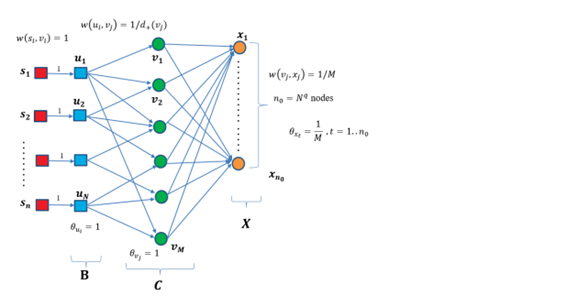
\includegraphics [scale=.5]{picture/Hinh3_3}
 				\end{center}
 				\caption{Giản thể từ bài toán SC về bài toán LSE.}
 				\label{refhinh3_3}
 			\end{figure}
 		\end{center}
 		\end {itemize}
 		{\bfseries Phân tích:} Qua bước xây dựng, ta thấy rằng | f$_{d}$(I,$\emptyset$) | = M + N. Nếu như có đỉnh bất kì u$_{i} \in$ B là đỉnh kề vào và v$_{j} \in$ C là đỉnh chưa bị lây nhiễm thì: 
 		\begin{center}
 			$\sum_{Các đỉnh hàng xóm tới đã bị lây nhiễm u}$ w(u, v$_{j}$) $\leq$ 1 - $\dfrac{1}{d_{in}(v_{j})}$ < 1 = $\theta_{v_{j}}$
 		\end{center}
 		
 		Do đó v$_{j}$ lầ đỉnh không bị lây nhiễm. Nếu không, các đỉnh trong C là các đỉnh không bị lây nhiễm.
 		
 		($\rightarrow$) Giả sử S' là lời giải của biểu diễn J$_{SC}$, có nghĩa là | S' | = t = k và nó phủ t phần tử $\vartheta$. Nếu ta chọn tập A chứa đỉnh u$_{i}$ tương ứng với S$_{i} \in$ S', với mọi đỉnh v$_{i} \in$ B kề với ít nhất một đỉnh trong A. Bằng bước phân tích trên, mọi đỉnh trong C là đỉnh không bị lây nhiễm. Ta có h$_{d}$(A) = t + M = k + M
 		
 		($\leftarrow$) Ngược lại, nếu J$_{LSE}$ có lời giải A, |A| $\leq$ k với h$_{d}$(I, A) $\geq$ k + M. Nếu A chứa t$_{1}$ (1 $\leq$ t$_{1}$ $\leq$ k) đỉnh trong C, h$_{d}$(I, A) $\leq$ k - t$_{1}$ + M < k + M. Do đó A không chứa bất kì đỉnh nào thuộc C. Ở đây, A $\subset$ B. Kết hợp với h$_{d}$(I, A) $\geq$ k + M, mọi đỉnh thuộc C là đỉnh không bị lây nhiễm. Do đó, mọi đỉnh u$_{i} \in$ A kề ít nhất với một đỉnh thuộc C. Vì vậy, qua bước xây dựng ta thấy rằng, S' = { S$_{i}$ | u$_{i} \in$ A } là lời giải cho bài toán J$_{1}$. Định lý được chứng minh.
 		
 		Bằng cách thay đổi một chút phương pháp chứng minh bên trên, ta có thể chứng minh thêm được một định lý về tính khó xấp xỉ của bài toán LSE.
 		
 		Định lý: Đánh giá xấp xỉ bài toán LSE với tỉ lệ n$^{1 - \varepsilon}$ trong mô hình T-DLT với mọi hằng số 0 < $\varepsilon$ < 1 là bài toán NP-khó .
 		
 		{\itshape Chứng minh}: Để chứng minh kết quả này, ta sử dụng phương pháp gap-introduction reduction \cite{vijay38} để chứng minh tính khó xấp xỉ của bài toán LSE. Sử dụng phép giản thể trong thời gian đa thức từ bài toán SC thành bài toán LSE , chúng tôi sẽ chỉ ra nếu tồn tại một thuật toán có thời gian đa thức có thể xấp xỉ được bài toán trên với tỉ lệ $^{1 - \varepsilon}$, thì sẽ tồn tại một thuật toán có thời gian đa thức để giải bài toán gốc.
 		
 		{\bfseries Xây dựng:} Cho một biểu diễn của bài toán SC, J$_{SC}$ = ($\vartheta$, S, t), ta xây dựng một biểu diễn J$_{LSE}$ = (G, I, d, k) 
 		\begin {itemize}
 			\item Tập các đỉnh và các cạnh: Với mỗi đỉnh v$_{j} \in$ C, ta thêm n$_{0}$ = N$^{q}$ đỉnh X = { x$_{1}$, x$_{2}$, ... , x$_{n_{0}}$} với một hằng số q đủ lớn và thêm một cạnh có hướng (v$_{j}$, x$_{l}$), l = 1 ... n$_{0}$.
 		
 			\item Ngưỡng lây nhiễm và trọng số: Gán w(v$_{j}$, x$_{l}$) = $\dfrac{1}{M}$; $\theta_{x_{l}}$ = $\dfrac{1}{M}$, l = 1 ... n$_{0}$.\\
 		\end {itemize}
 		Giả sử J$_{SC}$ có tập phủ đinh S' kích cỡ t, ta chọn tập A = ${{u_{i} | S_{i} \in S}}$. Qua bước phân tích, mọi đỉnh C đều là các đỉnh không bị lây nhiễm. Điều này dẫn tới mọi đỉnh trong X đều là các đỉnh không bị lây nhiễm. Bởi bước xây dựng này, ta có: | f$_{d}(I, \emptyset)$ | = N + M + N$^{q}$, | f$_{d}(I, A)$ | = N - k, do đó: 
 		\begin{center}
 			h(A) = | f$_{d}(I, \emptyset)$ | - | f$_{d}(I, A)$ | = M + N$^{q}$ + k
 		\end{center}
 		
 		Trong trường hợp J$_{SC}$ không có tập phủ đỉnh kích thước t, nó có ít nhất một đỉnh v$_{j}$ bị lây nhiễm. Điều này dẫn tới việc mọi trong X đều bị lây nhiễm. Do đó, | f$_{d}$(I, A) | > N - k + N$_{q}$ dẫn tới h(A) = M  + k < 2N.
 		
 		Lúc này giá trị của thuật toán có thể xấp xỉ bài toán LSE trong tỉ lệ n$^{1 - \varepsilon}$, ta chứng minh được rằng lời giải của bài toán SC có thể được tìm trong thời gian đa thức. Với bất kì biểu diễn J$_{SC}$ nào, ta xây dựng một biểu diễn J$_{LSE}$ theo cách xây dựng trên trong thời gian đa thức của m và n. 
 		
 		Trong trường hợp J$_{SC}$ có tập đỉnh phủ kích cỡ t, theo cách xây dựng của chúng tôi, lời giải tối ưu A$_{opt}$ của J$_{LSE}$ có h(A$_{opt}$) = k + M + N$_{q}$. Thuật toán xấp xỉ lời giải tối ưu với tỉ lệ n$^{1 - \varepsilon}$ (n = 2N + M + N$_{q}$ là số đỉnh của đồ thị đầu vào) do đó có thể tìm kiếm lời giải. 
 		
 			h(A(J$_{LSE}$)) $\geq$ $\dfrac{1}{n_{1 - \varepsilon}} h(A_{opt}) > \dfrac{1}{n^{1 - \varepsilon}}(M + N_{q} +k) = \dfrac{n^{\varepsilon}}{n}(M + N^{q} +k) > \dfrac{(M + N^{q} + k)^{\varepsilon}}{M + N^{q} + k}N^{q}$$> \dfrac{N^{q.\varepsilon}}{4N^{q}}N^{q} = \dfrac{1}{4}N^{q.\varepsilon}$. 
 		
 		Cho q đủ lớn để q > $\dfrac{ln(8N)}{\varepsilon.ln(N)}$, ta được: 
 		\begin{center}
			$h(A(J_{LSE})) > 2N$.
 		\end{center}
 	
 		Nếu $J_{LSE}$ không có tập phủ đỉnh kích cỡ t, thì tập tối ưu $A_{opt}$ của $J_{LSE}$ có 
 		\begin{center}
 			$h(A(J_{LSE})) < 2N$.
 		\end{center}
 	
 		Điều này cho thấy $J_{LSE}$ có một tập phủ đỉnh kích cỡ t khi và chỉ khi $h(A(J_{LSE})) < 2N$. Do đó ta có thể dùng A để giải quyết bài toán SC trong thời gian đa thức, hay P = NP. Điều này mâu thuẫn với giả thiết P $\neq$ NP.
 		
 		\subsubsection{Thuật toán nhanh và hiệu quả để giới hạn sự lây nhiễm thông tin (Fast And Effective Limiting Epidemics – FLE).}
 		Trong phần này, chúng tôi thiết kế một thuật toán heuristics có độ phức tạp thấp và kết quả rất khả quan. Trước khi bắt đầu, chúng tôi có định nghĩa một vài kí hiệu sẽ được sử dụng trong quá trình đề xuất thuật toán:
 		\begin {itemize}
 			\item t(u): vòng nhỏ nhất sao cho đỉnh u chuyển từ đỉnh không bị lây nhiễm sang đỉnh bị lây nhiễm.
 		
 			\item $a_{in}(u) = \sum_{I_{t(u) - 1} \bigcap N_{in}(u)} w(u,v):$ tổng trọng số các cạnh vào từ các đỉnh vào hàng xóm đã bị lây nhiễm trước vòng t(u).
 		
 			\item $\propto(u) = \sum_{v \in U^{d}_{i=t(u)+1}} I_{i} \bigcap N(u)$ w(u,v), i = t(u) + 1, ... , d: tổng trọng số các cạnh ra từ u tới các đỉnh bị lây nhiễm b tại vòng i.
 		
			\item $\beta(u): $ : số lượng các đỉnh ra, sao cho chúng chuyển từ bị lây nhiễm thành không bị lây nhiễm sau khi loại bỏ đỉnh u ra khỏi đồ thị.
		\end {itemize}
		Một cách trực quan, số lượng gia tăng các đỉnh được cứu $\delta(A, u)$ có thể xấp xỉ theo $\beta(u)$. Bên cạnh đó, để tăng cường tính hiệu quả của thuật toán đề xuất, chúng tôi kết hợp $\propto(u) và \beta(u)$ để tính toán khả năng lan truyền tin sai lệch của đỉnh u. Ý tưởng chính của thuật toán là chọn ra các đỉnh một cách lần lượt theo đánh giá của hai hàm $\propto và \beta$. Ban đầu, chúng tôi khởi tạo tập đỉnh được chọn A=$\emptyset$ và đặt tập các đỉnh được xét chọn U bằng với $V_{d}$. Trong mỗi bước, chúng tôi chọn ra đỉnh có trị số $\beta(u)$ lớn nhất trong đồ thị còn lại. Trường hợp tất cả các đỉnh đều có giá trị $\beta(u)$ là 0, chúng tôi chọn đỉnh có giá trị $\propto(u)$ cực đại. Thuật toán được mô tả ở hình \ref{refthuattoan1} sau.
		\begin{center}
			\begin{figure}[htp]
				\begin{center}
					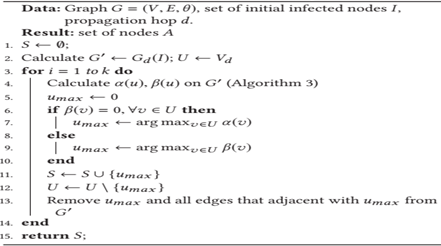
\includegraphics [scale=.65]{picture/thuattoan1}
				\end{center}
				\caption{Thuật toán nhanh và hiệu quả để giới hạn sự lây nhiễm thông tin}
				\label{refthuattoan1}
			\end{figure}
		\end{center}
	
		Khó khăn trong thuật toán chủ yếu đến từ bước tính toán các hàm $\propto và \beta$. Để giải quyết việc này, chúng tôi bắt đầu với ý tưởng tìm kiếm theo chiều rộng (Breath First Search - BFS) để tính toán $f_{d}(I)$ và dần dần cập nhật hàm $\propto_{in}()$. Sau đó, chúng tôi sử dụng nó để tính toán các hàm  $\propto và \beta$ theo định nghĩa của chúng. Thuật toán chi tiết được thể hiện trong hình \ref{refthuattoan2}
		\begin{center}
			\begin{figure}[htp]
				\begin{center}
					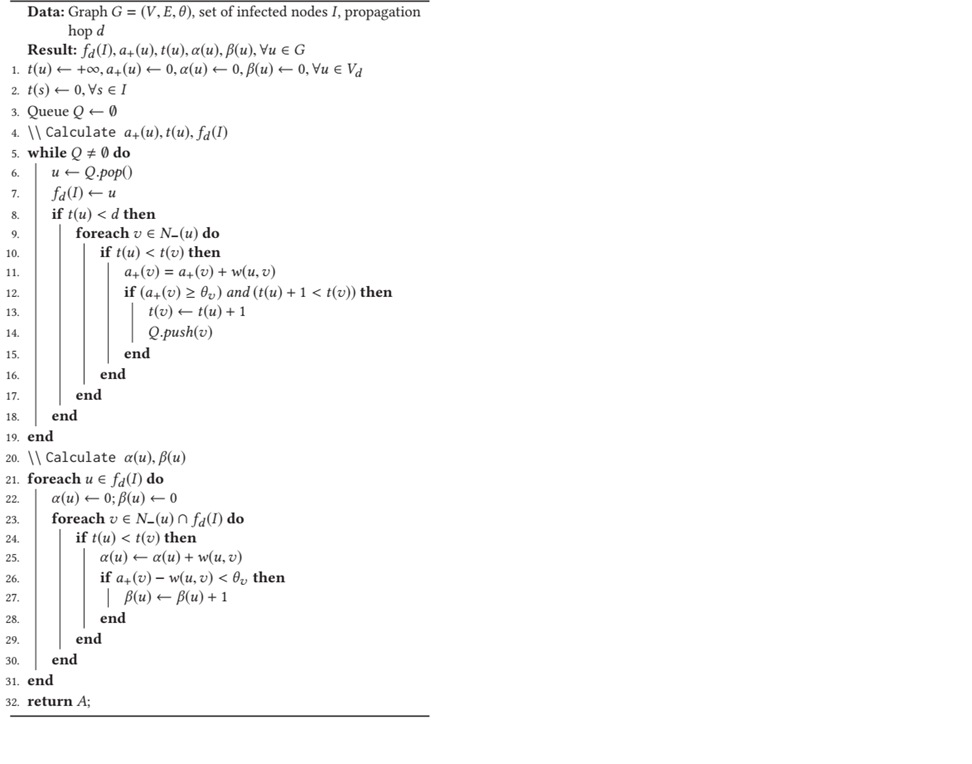
\includegraphics [scale=.5]{picture/thuattoan2}
				\end{center}
				\caption{Thuật toán tính $\propto() và \beta()$ có độ phức tạp $O(k(m_{d} + n_{d}))$}.
				\label{refthuattoan2}
			\end{figure}
		\end{center}
	
		{\itshape Chứng minh}: Để đánh giá độ phức tạp của thuật toán này, chúng ta cần đánh giá trước độ phức tạp của thuật toán. Ta dễ thấy rằng việc tính  toán $f_{d}(I)$ (dòng 5 - 19) có cách thức hoạt đông giống BFS. Do đó, độ phức tạp của nó là O($m_{d} và n_{d}$). Với bước tính toán $\propto(u) và \beta(u)$ (dòng 21 - 31), ta cần thăm tất cả các đỉnh trong $f_{d}(I)$ và tập các cạnh ra liền kề, do đó độ phức tạp của nó là O($m_{d} và n_{d}$). Do đó, độ phức tạp chung của thuật toán là O($m_{d} và n_{d}$). 
	\subsection{Giải pháp hạn chế Targeted Misinformation Blocking (Xác định và ngăn chặn thông tin sai lệch trên mạng xã hội)}
Với cách tiếp cận như cách Twitter đã làm năm 2016 là loại bỏ 125.000 tài khoản được nghi ngờ có liên quan đến các hoạt động khủng bố, hay như Facebook đã xóa 30.000 tài khoản giả mạo lan truyền các tin đồn trước cuộc bầu cử tổng thống Pháp năm 2017, giải pháp hạn chế Targeted Misinformation Blocking được đưa ra nhằm mục đích tìm những tài khoản cần loại bỏ khỏi mạng để nhằm làm hạn chế phát tán thông tin sai lệch.

\subsubsection{Định nghĩa bài toán}
Kí hiệu G=(V,E,w) là một đồ thị có hướng biểu diễn cho một mạng xã hội trên mô hình LT với V biểu diễn tập người dùng, E biểu diễn mối quan hệ giữa các cặp người người dùng, w là tập trọng số của các cạnh biểu diễn tần số tương tác giữa các người dùng. Gọi $N_{out}(v)$ và $N_{in}(v)$ lần lượt là tập đỉnh đi ra từ v và đi vào v. Mỗi cạnh có hướng (u,v) $\in$ E được gán một trọng số w(u,v) $\in$ [0,1] đảm bảo điều kiện $\sum_{u \in N_{in}(v)} \leq 1$.

Đưa ra một tập nguồn S = {$s_{1}, s_{2}, ... , s_{n}$}, $s_{i} \in V$ là tập tiềm năng phát tán thông tin sai lệch (tương tự như tập hạt giống trong bài IM \cite{kempe21}).

Trong mô hình LT, mỗi đỉnh v $\in$ V, có hai trạng thái active và inactive. Quá trình lan truyền trên mô hình LT được diễn tả như sau: Đầu tiên, mỗi đỉnh v được gán một trọng số ngẫu nhiên $\theta_{v} \in [0,1]$ thể hiện giá trị active của đỉnh kề u phải đạt được để có thể active v. Tiếp đến quá trình lan truyền diễn ra trong các vòng t = 1,2,3… như sau: 		
\begin {itemize}
\item Ở vòng 1, tất cả các đỉnh $s_{i} \in S$ ở trạng thái active và các đỉnh còn lại ở trạng thái inactive.

\item Ở vòng t $\ge$ 1, một đỉnh v ở trạng thái inactive được active nếu thỏa mãn điều kiện $$\sum_{\mbox{ $u \in N_{in}(v) $ và  u  là active}} w(u, v)\geq \theta_v$$

\item Khi một đỉnh ở trạng thái active thì sẽ luôn duy trì trạng thái đó trong suốt quá trình lan truyền thông tin. Quá trình lan truyền kết thúc khi không có đỉnh nào được active thêm.	
\end {itemize}

Kí hiệu $\sigma_{S}(G)$ là ảnh hưởng lan truyền của tập S trên đồ thị G dưới mô hình LT hay là số lượng đỉnh được active bởi nguồn S. Theo nghiên cứu của Kempe và các cộng sự đã chỉ ra rằng mô hình LT là tương đương với khả năng tiếp cận trong một đồ thị ngẫu nhiên g được gọi là đồ thị live-edge hoặc đồ thị mẫu. Trên mô hình LT, đồ thị live-edge được xây dựng như sau:
\begin {itemize}
\item Với mỗi v $\in$ V, chọn tối đa một cạnh đi vào nó một cách ngẫu nhiên, xác suất cạnh (u, v) được chọn là w(u, v).

\item Xác suất không có cạnh nào được chọn là 1 - $\sum_{u \in N_{in}(v)} w(u,v)$.
\end {itemize}

Cạnh được chọn gọi là cạnh sống (live-edge) và tất cả các cạnh khác gọi là cạnh bị chặn (blocked-edge). Chúng ta có xác suất tạo ra một đồ thị live-egde g từ G là:
\begin{align}
\Pr[g|G]=\prod_{v \in V}{p(v,g,G)}
\end{align}
với
\begin{equation}
p(v, g, G)= \left\{ \begin{array}{ll}
w(u, v), & \mbox{If $\exists u: (u, v) \in E_g$}\\
1-\sum_{u:(u, v) \in E}{w(u, v)}, & \mbox{Otherwise}\\
\end{array} \right.
\end{equation}

Ảnh hưởng lan truyền của nguồn S khi xóa bỏ các đỉnh trong tâp A trên đồ thị G[V$\backslash$A] kí hiệu là $\sigma_{S}(G \backslash A)$. Với A = $\emptyset$, trong \cite{kemple1} đã chỉ ra ảnh hưởng lan truyền của tập nguồn S trên G được tính bởi công thức:
\begin{align}
\sigma_S(G)=\sum_{g \in X_G}{\Pr[g|G]|R(g, S)|}
\label{inf_cal}
\end{align}
với $R(g, S)$ là tập các đỉnh đến được từ S trên g và $X_G$ là tập tất cả các đồ thị live-edge được tạo ra từ G. Đặc biệt, ảnh hưởng lan truyền của tập $S$ có thể được tính bằng đường đi đơn bắt đầu từ $u \in S$ theo công thức: 
\begin{align}
\sigma_{S}(G)=\sum_{x \in \mathsf{P}(G, S)} \prod_{e \in x}w(e)
\label{inf_path}
\end{align} 				
với $\mathsf{P}(G, S)$ là tập tất cả các đường đi đơn từ $s \in S$ tới bất kỳ đỉnh $v \in G \setminus \{S \cup \{s\} \} $ trên đồ thị G.		

\textbf{Phát biểu bài toán (Bài toán TMB):} Gọi G(V,E,w) là một đồ thị có hướng biểu diễn một mạng xã hội. Đưa ra một tập nguồn S = {$s_{1}, s_{2}, ... , s_{k}$}, S $\in$ V là tập tiềm năng phát tán thông tin sai lệch và một số nguyên $\gamma \leq | V |$ thể hiện cho số lượng người dùng tối thiểu chúng ta muốn đảm bảo thông tin sai lệch không lan truyền đến được họ.

\textbf{Yêu cầu:} Tìm tập đỉnh A $\in V \backslash S$ có ít đỉnh nhất sao cho khi xóa các đỉnh trong tập A khỏi đồ thị G thì đảm bảo h(A) = $\sigma_{S}(G) - \sigma_{S}(G \backslash A) \geq \gamma$, tức là đảm bảo ít nhất $\gamma$ người dùng không tiếp xúc với thông tin sai lệch.
\subsubsection{Độ phức tạp của bài toán}		
Trong mục này chúng tôi chỉ ra một số kết quả về độ khó của bài toán TMB trên mô hình LT.
\begin{theo}
	Cho nguồn tiềm năng phát tán thông tin sai lệch S dưới mô hình LT, bài toán TMB là $\#P-hard$ nếu S chỉ chứa 1 đỉnh.
\end{theo}
\begin{proof}
	Để chứng minh TMB là $\#P-hard$ chúng tôi sẽ chỉ ra độ khó của bài toán TMB là lớn hơn hoặc bằng với độ khó của bài toán $s$-$t$ paths mà đã được chứng minh có độ khó là $\#P-hard$ trong \cite{vali}. 
	\begin{define}[Bài toán $s$-$t$ paths \cite{vali}]
		Cho một đồ thị có hướng $G = (V, E), |V| = n, |E| = m$, bài toán s-t paths yêu cầu đếm số đường đi có hướng từ đỉnh $s$ tới đỉnh $t$ mà đi qua mọi đỉnh nhiều nhất một lần. 
	\end{define}			
	\begin{figure}[h]
		\begin{center}
			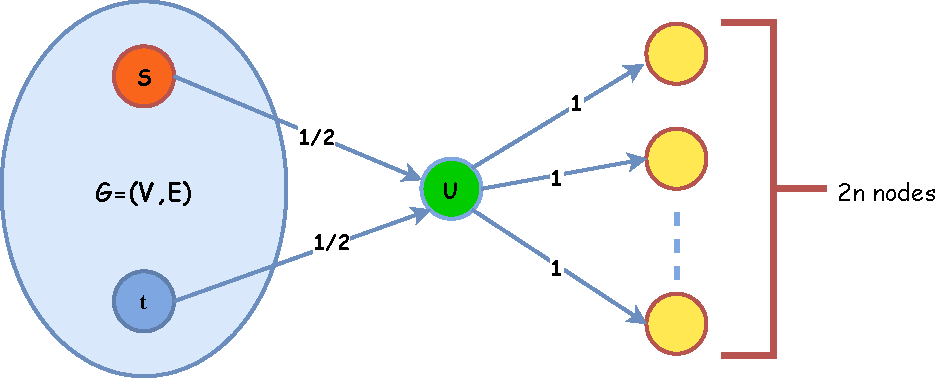
\includegraphics[height = 3 cm]{picture/reduce}
			\caption{Giản thể từ bài toán $s$-$t$ paths sang bài toán TMB.}
			\label{reduce}   
		\end{center}
	\end{figure}			
	Xem xét một thể hiện $\mathcal{I}_1$ của bài toán $s$-$t$ paths, với $G = (V, E), s, t$ cho trước. Như minh họa trong hình \ref{reduce}, từ G, chúng ta xây dựng G' như sau: Thêm đỉnh u và hai cạnh (s, u), (t, u) với trọng số $w(s, u) = w(t,u) = 1/2$, tiếp đó thêm tập $\mathcal{Q}$ gồm 2n đỉnh và kết nối u với chúng với trọng số là 1. Với các cạnh khác, thiết lập trọng số $w = 1/\Delta$, $\Delta$ là bậc vào lớn nhất của đồ thị G. Chúng ta chia tất cả các đường đi bắt đầu từ $s$ thành 2 nhóm: Tập tất cả các đường đi có đỉnh kết thúc thuộc tập $\mathcal{Q}$ và tập còn lại. Từ công thức \eqref{inf_path}, chúng ta có: 
	\begin{align}
	\sigma_{S}(G')&=\sum_{x \in \mathsf{P}(G', s)} \prod_{e \in x}w(e)= \sum_{v \in  G' \setminus Q} \left(  \sum_{x \in \mathsf{P}(G', s, v)} \prod_{e \in x}w(e) \right) + \sum_{v \in Q} \left(  \sum_{x \in \mathsf{P}(G', s, v)} \prod_{e \in x}w(e) \right)  \nonumber
	\\
	&  =\sum_{x \in \mathsf{P}(G, s)} \prod_{e \in x}w(e) + \sum_{x \in \mathsf{P}(G', s, u)} \prod_{e \in x}w(e) + \sum_{v \in   Q } \left(  \sum_{x \in \mathsf{P}(G', s, v)} \prod_{e \in x}w(e)  \right)  \nonumber
	\\
	& = \sigma_{S}(G) +  \sum_{x \in \mathsf{P}(G', s, u)} \prod_{e \in x}w(e) +  \sum_{v \in Q } \left(  \sum_{x \in \mathsf{P}(G', s, v)} \prod_{e \in x}w(e)  \right) 
	\label{eq_1}
	\end{align}  
	và, 
	\begin{align}
	\sum_{v \in  Q } \left(  \sum_{x \in \mathsf{P}(G', s, v)} \prod_{e \in x}w(e)  \right) &= \sum_{v \in Q} \left(  \sum_{x \in \mathsf{P}(G', s, u)} w(u, v)  \prod_{e \in x}w(e)  \right) \nonumber
	\\
	& =\sum_{v \in Q} \left(  \sum_{x \in \mathsf{P}(G', s, u)} \prod_{e \in x}w(e)  \right)\ \ \ \mbox{(Vì $w(u, v)=1$)} \nonumber
	\\
	& = 2n \cdot \sum_{x \in \mathsf{P}(G', s, u)} \prod_{e \in x}w(e)
	\label{eq_3}
	\end{align}
	Từ \eqref{eq_1} và \eqref{eq_3}, chúng ta thu được:
	\begin{align}
	h(u)&= \sigma_{S}(G')- \sigma_{S}(G'\setminus \{u\})=  \sigma_{S}(G')- \sigma_{S}(G)=(2n+1)\cdot \sum_{x \in \mathsf{P}(G', s, u)} \prod_{e \in x}w(e)
	\\
	& = (2n+1)\cdot \left(  w(s, u)+ \sum_{x \in \mathsf{P}(G, s, t)} w(t, u) \prod_{e \in x}w(e) \right) 
	\\
	& = (2n+1)\cdot \left(  \frac{1}{2}+ \frac{1}{2} \sum_{x \in \mathsf{P}(G, s, t)}  \prod_{e \in x}w(e) \right)  \ \ \ \mbox{(Vì $w(s, u)= w(t, u)=\frac{1}{2}$)}
	\\
	& = \frac{2n+1}{2} \left(  \sum_{x \in \mathsf{P}(G, s, t)}  \prod_{e \in x}w(e) +1 \right) 
	\\
	& = \frac{2n+1}{2} \left(  \sum_{i=0}^{n-1} \alpha_i w^i +1 \right) 
	\end{align}   		
	với $\alpha_i=|\mathsf{P}_i(G, s, t)|$. Đặt $f(w)=\sum_{i=0}^{n-1}\alpha_i w^i$. Từ cấu trúc liên kết của G', chúng ta thấy rằng $h(u)=\max_{v \in G'}h(v)$ và $0 \leq  f(w) < 1$. Nếu có thể xác định $f(u) \geq \beta$ với $\forall \beta \in [0, 1]$ trong thời gian đa thức thì chúng ta sẽ giải được bài toán $s$-$t$ paths trong thời gian đa thức. Sử dụng tìm kiếm nhị phân trên đoạn [1, $\Delta^{n-1}$] chúng ta có thể xác định được giá trị của $f(w)$. Yêu cầu này được thực hiện trong $\mathcal{O}(\log(\Delta^{n-1}))=\mathcal{O}((n-1)\log\Delta) =\mathcal{O}(n\log n)$. Do đó việc tính toán $f(u)$ có thể thực hiện trong thời gian đa thức. Tiếp đến thay đổi trọng số w thành n giá trị 
\end{proof}
\subsubsection{Thuật toán đề xuất}
{\itshape Thuật toán tham lam (Greedy algorithm)}
Trong phần này chúng tôi giới thiệu một thuật toán xấp xỉ đảm bảo tỉ lệ 1 + ln($\gamma / \varepsilon$) dựa vào tính chất submodular và tính đơn điệu của hàm h(A). 		
\\
\begin{algorithm}[tbh]			
	\SetNlSty{text}{}{.}
	%\SetAlgoNlRelativeSize{0}
	\KwData{Graph $G=(V,E, w)$,  $S=\{s_1, s_2, .., s_k\}$, threshold $<\gamma < |V|$, parameter $\epsilon \in (0, \gamma)$} 
	\KwResult{set of nodes $A$}
	$A \leftarrow \emptyset$;
	\\
	\While{$h(A) < \gamma-\epsilon $}
	{ 	
		$u=\arg \max_{v \in V\setminus \{A \cup S\}} {h(A+ \{v\})- h(A)}$; 
		\\
		$A \leftarrow A \cup \{u\}$;
	}
	\Return $A$;
	\caption{Greedy Algorithm (GA)}
	\label{GA}
\end{algorithm}

\begin{theo}					
	Hàm $h(\cdot)$ là hàm submodular và monotone. 
	\label{sub}
\end{theo}	

\begingroup
\fontsize{13pt}{12pt}
\selectfont		 
\begin{proof}	
	Kí hiệu $N_E(A)$ là tập tất cả các cạnh (u, v) với u, v $\in$ $A$. Theo định lý 5 trong \cite{khali}, cho $A \subseteq T$ chúng ta có $h(T)-h(A)=\sigma_{S}(N_E(A))- \sigma_{S}(N_E(T)) \geq 0$. Do đó $h(\cdot)$ là một hàm monotone. 
	Tiếp đến chúng ta chỉ ra rằng $\sigma_S(G \setminus A)$ là một hàm submodular với $A$ là biến số. Đặt $E_{T, v}=N_E(T+\{v\})\setminus N_E(T), E_{A, v}= N_E(A+\{v\}) \setminus N_E(A)$ dễ thấy $E_{T, v} \subseteq E_{A, v}$  và vì thế $A \subseteq T$ $\Rightarrow$ $N_E(A)\cup E_{T, v} \subseteq N_E(A+ \{v\})$. Lấy $\sigma_S(G \setminus X)$ là ảnh hưởng lan truyền của tập $S$ trên đồ thị $G$ sau khi loại bỏ tập cạnh $X \subset E$, chúng ta thu được $\sigma_{S}(G \setminus A)=\sigma_{S}(G \setminus N_E(A)$. Theo định lý 6 trong \cite{khali}, $\forall X \subseteq Y, e \in Y\setminus X$, chúng ta có: 
	\begin{align}
	\sigma_{S}(G \setminus (X \cup \{e\}) - \sigma_{S}(G \setminus X) 
	\leq \sigma_{S}(G \setminus (Y \cup \{e\})) - \sigma_{S}(G \setminus Y)
	\label{super}
	\end{align}
	Therefore,
	\begin{align}
	\sigma_{S}(G \setminus A)-\sigma_{S}(G \setminus (A \cup \{u\})) 
	& =\sigma_{S}(G \setminus N_E(A))-\sigma_{S}(G \setminus N_E(A+\{v\})) 
	\\
	&	\geq \sigma_{S}(G \setminus N_E(A))-\sigma_{S}(G \setminus (N_E(A) \cup E_{T, v})) 
	\\
	&	\geq \sigma_{S}(G \setminus N_E(T))-\sigma_{S}(G \setminus (N_E(T) \cup E_{T, v}))  
	\\
	& = \sigma_{S}(G\setminus T)-\sigma_{S}(G \setminus (T \cup \{u\}))  ( \mbox{Apply the inequality  \eqref{super}})
	\end{align}
	Combine with $h(A)= \sigma_S(G)- \sigma_S(G\setminus A)$ we easy see that $h(\cdot)$ is a supmodular function.
\end{proof}
\endgroup

\begin{theo} Với $\forall$ $\epsilon \in (0, \gamma)$, thuật toán \ref{GA} đưa ra lời giải $A$ thỏa mãn $h(A) \geq \gamma- \epsilon$, và $|A|$ là không vượt quá tích của $1+\ln(\gamma/ \epsilon)$ với số đỉnh của lời giải tối ưu \label{app}
\end{theo}		
\begin{proof}
	Chi tiết cách chứng minh định lý \ref{app} được chỉ ra trong \cite{snam}. 
\end{proof}
{\itshape Thuật toán TMB (TMB algorithm)}
Thuật toán tham lam đưa ra một lời giải tốt xong lại không đảm bảo yêu cầu về thời gian với dữ liệu lớn do đó trong phần này chúng tôi đưa ra một giải pháp đảm bảo yêu cầu cả về độ tốt cũng như thời gian tính toán. Dưới đây là các bước chính trong thuật toán chúng tôi đề xuất:
\begin {itemize}
\item Đầu tiên sáp nhập các đỉnh trong tập nguồn S thành một nút I bằng cách áp dụng thuật toán 2 được đề xuất bởi Zhang \cite{zhang39}. Chúng ta thu được một đồ thị mới và nguồn phát tán thông tin sai lệch bây giờ chỉ là một đỉnh I duy nhất.

\begin{algorithm}[tbh]			
	\KwData{Graph $G=(V,E, w)$,  $S=\{s_1, s_2, .., s_k\}$} 
	\KwResult{Graph $G'=(V', E', w')$, I}
	$G' \leftarrow G$;
	\\
	Add node I to G'			
	\\
	\ForEach{s $\in$ S}
	{
		\If{$\exists$ (s, v) }
		{
			\eIf{(I, v) $\notin$ G'}
			{
				Add edge (I, v) to G'
				\\
				w'(I, v) = w(s, v)
			}
			{
				w'(I, v) = w'(I, v) + w(s, v)
			}
			Remove (s,v) from G'
		}
	}
	Remove all node in S from G'
	\\
	\Return G', I;
	\caption{MERGE Algorithm(MERGE)}
	\label{MERGE}
\end{algorithm}		

\item Tiếp đến chúng tôi tạo ra $\mu(\mu \in N*)$ đô thị mẫu g từ G bằng cách: mỗi đỉnh v $\in$ V chọn nhiều nhất một đỉnh kề đi đến nó môt cách ngẫu nhiên sao cho xác suất chọn cạnh (u, v) là w(u, v) và xác suất không chọn cạnh nào là 1 - $\sum_{u} w(u, v)$. Những cạnh được chọn được gọi là cạnh sống  (live - edge) và tất cả các cạnh còn lại được gọi là cạnh bị chặn (blocked-edge). Chi tiết cách lấy đồ thị mẫu được mô tả trong thuật toán \ref{GSGLT} và trong hình \ref{example}:
\begin{algorithm}
	\KwData{Graph G=(V,E, w), I} 
	\KwResult{Tree g root at I}			
	g $\Leftarrow \emptyset$
	\\
	\For{$v \in V_G$}
	{	
		$\gamma_{active} \leftarrow$ random(0, 1)
		\\
		sum\_weight $\leftarrow$ 0
		\\
		\For{u $\in$ in\_neighbors(v)}
		{
			sum\_weight += w(u, v)
			\\
			\If{sum\_weight $\geq \gamma_{active}$}
			{
				Add edge (u, v) to g
				\\
				Break
			}
		}
	}		
	g $\leftarrow$ DFS$_{tree}$(I,g)
	\\
	\Return g
	\caption{Get Sample Graph LT Algorithm (GSG\_{LT})}
	\label{GSGLT}
\end{algorithm}	
\begin{figure}[h]
	\subfloat[Đồ thị $G'$ sau khi hợp nhất các đỉnh trong nguồn S\label{fig:test1}]
	{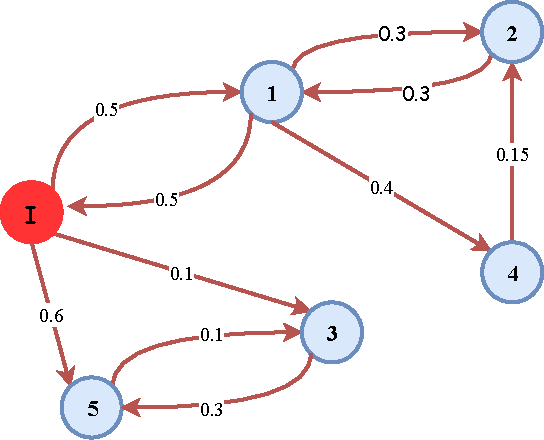
\includegraphics[width=.3\linewidth]{picture/1}}\hfill
	\subfloat[Một đồ thị mẫu $g$\label{fig:test2}]
	{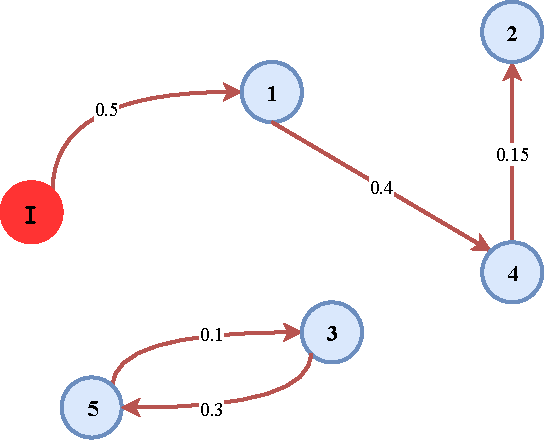
\includegraphics[width=.3\linewidth]{picture/2}}\hfill
	\subfloat[Một cây gốc $I$ tạo ra từ $G$ \label{fig:test3}]
	{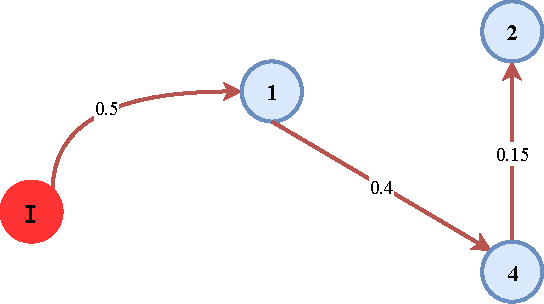
\includegraphics[width=.3\linewidth]{picture/3}}
	\caption{Ví dụ tạo ra một cây gốc $I$ từ $G$ trên mô hình LT}
	\label{example}
\end{figure}			
\item Trên cây T$_{I}^i$, ảnh hưởng địa phương của nút v là số nút con của cây gốc v kể cả v trên cây T$_{I}^i$. Áp dụng thuật toán DFS dễ dàng tìm được số nút con của v. Ảnh hưởng giảm của nguồn S khi loại đỉnh u khỏi G bằng lượng ảnh hưởng giảm trung bình khi loại u trên tất cả các cây T$_{I}^i$. Kí hiệu h(u, $T_I^i$) là lượng ảnh hưởng giảm trên cây $T_I^i$ sau khi loại bỏ đỉnh u khỏi $T_I^i$. Áp dụng phương pháp Lazy forward của Leskovec \cite{krause} để tìm kiếm lời giải. 
\begin{algorithm}[h]
	%\SetAlgoNlRelativeSize{0}
	\KwData{Graph $G=(V,E, w)$,  $\mathcal{S}=\{s_1, s_2, .., s_q\}$, threshold $\gamma>0$} 
	\KwResult{set of nodes $A$}
	$A \leftarrow \emptyset$;	$(G', I) \leftarrow \mathtt{Merge}(G, \mathcal{S})$.
	\\
	Remove all node, $I$ can't reach in $G$.
	\\
	Generate $\eta$ sample graphs and set $\eta$ trees $\mathcal{L}=\{T_{I}^1, T_{I}^2, \ldots, T_{I}^{|\mathcal{\eta}|}\}$
	\\
	For each $ T_{I} \in \mathcal{L}$, calculate $h(u, T_{I})$ for all $u \in T_{I}$ (by using DFS algorithm).
	\\
	\For{$u \in V$}
	{
		$u.\delta(u) \leftarrow \frac{1}{\eta}\sum_{T_{I} \in \mathcal{L}} h(u, T_{I})$; $u. cur \leftarrow 1$
		\\
		Insert element $u$ into $Q$ with $u.\delta(u)$ as the key
	}
	$ h_{max} \leftarrow 0$; $iteration \leftarrow 1$
	\\
	\While{$ h_{max} <\gamma-\epsilon $}
	{
		$u_{max} \leftarrow  dequence \  Q$
		\\
		\eIf{$u_{max}.cur =iteration$}
		{
			$A \leftarrow A \cup \{u_{max}\}$ ; $iteration \leftarrow iteration+1 $
			\\
			\ForEach{$T_{I} \in \mathcal{L}_c $}
			{
				If $u_{max} \in T_{I}$, remove node $u_{max}$ and update $h(v, T_{I})$, $ \forall v \in T_{I}$.
			}
			$h_{max} \leftarrow h_{max}+ u_{max}.\delta(u_{max})$
		}
		{
			$u_{max}. \delta(u_{max}) \leftarrow  \frac{1}{\eta}\big(\sum_{T_{I} \in \mathcal{L}}h(I, T_{I}) - \sum_{T_{I} \in \mathcal{L}} h(I, T_{I} \setminus u_{max})\big)$
			\\
			$u_{max}. cur =iteration$; re-insert $u_{max}$ into $Q$
		}
	}
	\Return $A$;
	\caption{Scalable $\mathsf{TMB}$ for LT model ($\mathsf{TMB}$) Algorithm}
	\label{STMB}
\end{algorithm}				
\end {itemize}
{\itshape Độ phức tạp của thuật toán: }		
Để đánh giá độ phức tạp của thuật toán trước tiên chúng ta đi phân tích độ phức tạp của các thuật toán con trong nó.
\begin {itemize}
\item Thuật toán MERGE có độ phức tạp là O(k + | N$_{in}(S)$ |).

\item Quá trình tạo ra $\mu$ đồ thị mẫu dòng 3 có độ phức tạp O($\mu(m + n)$).

\item Do T$_{I}^i$ là một cây nên việc tính toán h(u, T$_{I}^i$) $\forall u \in T_{I}^i$ mất O$(\mu n)$ 

\item Phần Lazy Forward có độ phức tạp là O(qmn) với q là số vòng lặp từ dòng 10 đến 23.
\end {itemize}
Vậy nên toàn bộ thuật toán TMB có độ phức tạp là O($\mu$(m+qn)).
	
	\subsection{ Áp dụng các giải pháp đề xuất trên dữ liệu thực}
	Trong phần này nhóm tác giả đưa ra kết quả thực nghiệm của giải hai giải pháp chỉ ra trong mục trước trên dữ liệu có sẵn và dữ liệu thu thập được, từ đó để thấy được hiệu quả của phương pháp nhóm đề xuất.
		
		\subsubsection{Giải pháp Limiting the spread of epidemics within time constraint on online social network}
		{\itshape - Dữ liệu có sẵn}
		
		Trong phần này, chúng tôi thực nghiệm trên một số MXH trực tuyến để kiểm chứng tính hiệu quả của thuật toán khi so sánh nó với các thuật toán cơ sở được sử dụng trong các bài toán lan truyền thông tin \cite{nguyen30}, \cite{kempe21}, \cite{zhang40}. Chúng tôi so sánh đánh gia trên ba yêu tố chính: chất lượng lời giải, tính mở rộng, tác động của số vòng lan truyền d trên một vài các MXH trực tuyến thực tiễn. Các thuật toán cơ sở sẽ sử dụng bao gồm:
		\begin {itemize}
			\item Random: Thuật toán chọn ngẫu nhiên k đỉnh trong N$_{d}(S)$.
		
			\item Maxdegree (Maxdeg): Thuật toán heuristic chọn lần lượt các đỉnh có bậc cao nhất trong tập V$_{d}$ cho đến khi đủ k đỉnh.
		
			\item Greedy: Thuật toán heuristic chọn lần lượt k đỉnh, trong mỗi lần chọn sẽ chọn ra đỉnh sao cho khi loại bỏ đỉnh đó sẽ cứu được nhiều đỉnh nhất có thể.
		\end {itemize}
		Chúng tôi thực nghiệm sử dụng một hệ thống máy có cấu hình sau: Intel(R) Core(TM) i5-6200U CPU @ 2.30 GHz (up to 2.40 GHz), bộ nhớ RAM 4GB, ngôn ngữ lập trình C++.
		
		{\itshape - Dữ liêu:}
		
		 Chúng tôi thực nghiệm thuật toán trên nhiều bộ dữ liệu thực tế khác nhau. Bên cạnh việc lựa chọn các bộ dữ liệu để đảm bảo sự đa dạng về kích thước, chúng tôi cũng lựa chọn nhiều miền dữ liệu khác nhau, bảng ... thể hiện các bộ dữ liệu nhóm tác giả sử dụng.
		\begin{table}
			\centering
			\begin{tabular}{|c|c|c|c|c|}
				\hline 
				Mạng & Số đỉnh & Số cạnh & Loại & Bậc trung bình \\ 
				\hline 
				Gnutella & 6,301 & 20,777 & Có hướng & 3.29 \\ 
				\hline 
				Wikipedia vote & 7,115 & 103,689 & Có hướng & 14.57 \\ 
				\hline 
				Amazon & 262,111 & 1,234,877 & Có hướng & 4.71 \\ 
				\hline 
				Google web & 875,713 & 5,105,039 & Có hướng & 5.83 \\ 
				\hline 
			\end{tabular} 
			\caption{Các bộ dữ liệu}
		\end{table}
		
		{\itshape Các thiết lập} Chúng tôi sử dụng các thiết lập dưới đây cho việc đánh giá thực nghiệm:
		
		- Trọng số của cạnh: w(u,v) = 



